\documentclass[11pt,oneside]{article}

\usepackage{setspace,graphicx,amssymb,amsmath,latexsym,amsfonts,amscd,amsthm,multirow,ctable,mathdots,caption,array}
\usepackage{fancyhdr,tabularx,cite,mathrsfs,mathtools}
\usepackage[headings]{fullpage} \usepackage{stmaryrd}
%\usepackage[all]{xy}
\usepackage{rotating}

\usepackage{hyperref}

\usepackage{subcaption}

\usepackage{adjustbox} \usepackage{fancybox}
%------------------------------------------------------------------%




%------------------------------------------------------------------%

\newcommand{\bea}{\begin{eqnarray}} 
\newcommand{\eea}{\end{eqnarray}} 
\newcommand{\bee}{\begin{eqnarray*}} 
\newcommand{\eee}{\end{eqnarray*}} 
\newcommand{\al}{\begin{align*}} 
\newcommand{\eal}{\end{align*}} 
\newcommand{\be}{\begin{equation}} 
\newcommand{\ee}{\end{equation}} 
\newcommand{\eq}[1]{(\ref{#1})} 
\newcommand{\bem}{\begin{pmatrix}} 
\newcommand{\eem}{\end{pmatrix}} 


\def\a{\alpha} 
\def\b{\beta} 
\def\c{\gamma} 
\def\d{\delta} 
\def\dbar{\bar{\partial}} 
\def\e{\epsilon}    
\def\f{\phi}  
\def\vf{\varphi}   

\def\h{\eta} 
\def\i{\iota} 
\def\im{\mathrm{Im}} 
\def\mm{^{(m)}}
\def\inf{\infty} 
\def\j{\psi} 
\def\k{\kappa}
\def\l{\lambda} 
\def\m{\mu} 
\def\n{\nu} 
\def\na{\nabla} 
\def\o{\omega}  
\def\w{\omega} 
\def\p{\pi}    
\def\pa{\partial}        
\def\re{\mathrm{Re}}
\def\r{\rho}                  
\def\s{\sigma}            
\def\t{\tau} 
\def\th{\theta} 
\def\til{\tilde} 
\def\u{\upsilon} 
\def\v{\varphi} 
\def\x{\xi} 
\def\we{\wedge} 
\def\z{\zeta} 
\def\zb{\bar{z}} 
\def\D{\Delta} 
\def\F{\Phi} 

\def\J{\Psi} 
\def\L{\Lambda} 
\def\O{\Omega} 
\def\P{\Pi} 
\def\Q{\Theta} 
\def\Sig{\Sigma} 
\def\T{\Theta} 
\def\Tr{\tr} 
\def\U{\Upsilon} 
\def\X{\Xi} 

\def\odd{{\rm odd}}
\def\even{{\rm even}}

\newcolumntype{R}{ >{$}r <{$}}
\newcolumntype{C}{ >{$}c <{$}}
\newcolumntype{L}{ >{$}l <{$}}
\newcolumntype{F}{>{\centering\arraybackslash}m{1.5cm}}

\def\ll{\ell}
\def\LL{\Lambda}

\def\ch{\rm ch}

\newcommand{\gt}[1]{\mathfrak{#1}}
\newcommand{\mc}[1]{\mathcal{#1}}
\newcommand{\tl}[1]{\tilde{#1}}
\newcommand{\wtl}[1]{\widetilde{#1}}
\newcommand{\comment}[1]{}



% Standard sets and objects
\newcommand{\RR}{{\mathbb R}}%Reals
\newcommand{\RRm}{\RR^{\times}}%non-zero real
\newcommand{\RRp}{\RR^+}%positive real
\newcommand{\CC}{{\mathbb C}}%Complex
\newcommand{\CCm}{\CC^{\times}}%non-zero complex
\newcommand{\PP}{{\mathbb P}}%Projective
\newcommand{\ZZ}{{\mathbb Z}}%Integers
\newcommand{\ZZp}{\ZZ^+}%Positive integers
\newcommand{\ZZm}{\ZZ^{-}}%Negative integers
\newcommand{\ZZx}{\ZZ^{\times}}%non-zero integers
\newcommand{\N}{{\mathbb N}}%Natural numbers
\newcommand{\QQ}{{\mathbb Q}}%Rationals
\newcommand{\QQm}{{\mathbb Q}^{\times}}%non-zero rationals
\newcommand{\QQp}{{\mathbb Q}^+}%positive rationals
\newcommand{\QQc}{\overline{\QQ}}%Algebraic closure of the rationals
\newcommand{\OO}{{\mathbb O}}%Octonions
\newcommand{\HH}{{\mathbb H}}%quaternions
\newcommand{\FF}{{\mathbb F}}%finite field

\newcommand{\cI}{\mathcal{I}}

\newcommand{\hh}{{\mathbf h}}%hyperbolic plane
\newcommand{\kk}{{\mathbf k}}%infinite field
\newcommand{\kkm}{\kk^{\times}}
\newcommand{\kkp}{\kk^+}
\newcommand{\ii}{{\bf i}}%Sqrt of -1
\newcommand{\diff}{{\rm d}} %Differential
\newcommand{\uu}{{\bf 1}}   %Bold unit
\newcommand{\GGa}{{\mathbb G}_a}%One dimensional additive group
\newcommand{\GGm}{{\mathbb G}_m}%One dimensional multiplicative group

\newcommand{\tpi}{2\pi\ii}%The fundamental constant
\newcommand{\fps}{4\pi^2}%minus the fundamental constant squared

\newcommand{\tc}{\!\!:\!\!}     %A tight colon
\newcommand{\lab}{{\langle}}    %Left angle brackets
\newcommand{\rab}{{\rangle}}    %Right angle brackets

% Standard operators
\newcommand{\End}{\operatorname{End}}
\newcommand{\Aut}{\operatorname{Aut}}
\newcommand{\Inn}{\operatorname{Inn}}
\newcommand{\Out}{\operatorname{Out}}
\newcommand{\Span}{\operatorname{Span}}
\newcommand{\Der}{\operatorname{Der}}
\newcommand{\Lie}{\operatorname{Lie}}
\def\jac{\operatorname{j}}

\def\infm{\operatorname{inf}}
\def\supr{\operatorname{sup}}

\newcommand{\wt}{\operatorname{wt}}
\newcommand{\Id}{\operatorname{Id}}
\newcommand{\tr}{\operatorname{{tr}}}
\newcommand{\str}{\operatorname{{str}}}
\newcommand{\Res}{\operatorname{Res}}
\newcommand{\Ind}{\operatorname{Ind}}
\newcommand{\Gal}{\operatorname{Gal}}
\newcommand{\Fix}{\operatorname{Fix}}
\newcommand{\Ann}{\operatorname{Ann}}
\newcommand{\Lifta}{\operatorname{Lift}_{\rm add}}
\newcommand{\Liftm}{\operatorname{Lift}_{\rm exp}}
\newcommand{\Sym}{{\textsl{Sym}}}
\newcommand{\Alt}{{\textsl{Alt}}}
\newcommand{\Dih}{{\textsl{Dih}}}
\newcommand{\HO}{{\textsl{Oct}}}
\newcommand{\Div}{\operatorname{Div}}
\newcommand{\sgn}{\operatorname{sgn}}
\newcommand{\ex}{\operatorname{e}} %Number theory exp
\newcommand{\vol}{\operatorname{vol}}
\newcommand{\ad}{\operatorname{ad}}
\newcommand{\sdim}{\operatorname{sdim}}

\newcommand{\ten}{{T}}	%Tensor algebra
\newcommand{\sym}{\operatorname{\wedge}}	%Symmetric algebra
\newcommand{\alt}{\operatorname{\vee}}	%Alternating algebra

% Groups
\newcommand{\PSL}{\operatorname{\textsl{PSL}}}    %PSL group
\newcommand{\SL}{\operatorname{\textsl{SL}}}      %SL group
\newcommand{\Sp}{\operatorname{\textsl{Sp}}}      %Sp group
\newcommand{\PGL}{\operatorname{\textsl{PGL}}}    %PGL group
\newcommand{\AGL}{{\textsl{AGL}}}    %AGL group
\newcommand{\GL}{{\textsl{GL}}}      %GL group
\newcommand{\SU}{\operatorname{\textsl{SU}}}    %SU group
\newcommand{\SO}{\operatorname{\textsl{SO}}}    %SO group

% Speedy greek
\newcommand{\vn}{V^{\natural}} %Moonshine module
\newcommand{\ogi}{\theta}     %Kummer involution
\newcommand{\cas}{\omega}	%Casimir element
\newcommand{\G}{\Gamma}	%Gamma
\newcommand{\g}{\gamma}	%gamma

% Custom objects
\newcommand{\chs}{{\rm ch}_0}
\newcommand{\chl}{{\rm ch}_L}
\newcommand{\dd}{d}
%\newcommand{\rs}{{\sf R}}	%deep hole root system
\newcommand{\rs}{{X}}	%deep hole root system
\newcommand{\wttwo}{{ F}}
\newcommand{\MM}{\mathbb{M}}	%monster group
\newcommand{\Co}{\textsl{Co}}	%Conway group

\newcommand{\bP}{\textbf{P} }
\newcommand{\bV}{\textbf{V} }
\newcommand{\bT}{\textbf{T} }
%------------------------------------------------------------------%

%Math environments
\newtheorem{thm}{Theorem}[section]
\newtheorem{cor}[thm]{Corollary}
\newtheorem{lem}[thm]{Lemma}
\newtheorem{prop}[thm]{Proposition}
\newtheorem{conj}[thm]{Conjecture}

\theoremstyle{definition}
\newtheorem{defn}[thm]{Definition}

\theoremstyle{remark}
\newtheorem{rmk}[thm]{Remark}
%\newtheorem*{rmk}{Remark}

\numberwithin{equation}{section}
%\numberwithin{equation}{subsubsection}
\newtheorem*{eg}{Example}


%------------------------------------------------------------------%

\pagestyle{fancy}

\addtolength{\headheight}{1.7pt}

\fancyhf{} \fancyhead[C]{\textsc{{A} semi-technical overview of zk-{S}narks and {S}onic for Veil}}

\fancyhead[R]{\thepage}
\renewcommand{\headrulewidth}{0.3pt}

\graphicspath{ {./} }


%------------------------------------------------------------------%


\begin{document}

\setstretch{1.4}

\title{ \vspace{-35pt} \textsc{\huge{{A} semi-technical overview of zk-{S}narks
and {S}onic\\} } }

\renewcommand{\thefootnote}{\fnsymbol{footnote}}
\renewcommand{\thefootnote}{\arabic{footnote}} 

\author{ Paul de Lange\footnote{{\em email:} {\tt
p.delange@uky.edu} } }

\maketitle

\abstract{

draft

}

\clearpage

\tableofcontents

\clearpage

%------------------------------------------------------------------%
\section{Introduction}\label{sec:intro}
%------------------------------------------------------------------%
This document aims at explaining how Sonic works, what is does and how it can be
implemented. We intend to be pragmatic over academic and will try to only introduce
formal concepts when they are needed. Some common concepts and buzzwords are briefly
explained in info boxes.

\clearpage

\section{My first Sigma protocol}
Valery is having an existential crisis. She's color blind, but she is starting to
believe that maybe she really isn't, and that all her friends and family are
just conspiring to trick her into believing she is.\\
Along comes Peter, her uncle, and Alice starts ventilating her conspiracy theory
to him.\\ \\
\bV: I trust you all no longer; I don't believe you can distinguish
between what you call `blue' and `red' any better than I can. Unless you can
offer me some proof.\\
\bP: Got it.\\
Peter takes out of his pocket two balls: one that's red, the other blue. Valery
however, being color blind, sees two identical balls.\\
\bP: You see these two balls, and you can confirm they are identical?\\
\bV: Yes, indeed.\\
\bP: Let me convince you that I \emph{can} distinguish between them.
I will hand over the balls to you now. I want you to take one ball
in each hand, and then hold the balls behind your back, so I can not see them.
Then, I need you to decide yourself whether you swap the balls or not. After
that, you present the balls to me again. Now, since I claim I can distinguish
the balls, I should easily be able to tell whether you swapped the balls or not.
However, in case I too see two identical balls, and can not see color as you
suspect, I will not be able to tell whether you made the swap, and I won't be
able to see.\\
Peter hand over the balls, blue in Valery's left hand; red in her right. Valery,
per instruction, places the balls behind her back and decides to swap them. She
presents the balls back to Peter.\\
\bP: You swapped them.\\
\bV: I did! OK, maybe you are right after all!
\\ \\
We have just witnessed our very first interactive proof of
knowledge\footnote{Such a protocol is more abstractly referred to as a Sigma
protocol, as the exchange $\bP \rightarrow \bV \rightarrow \bP$ can be drawn to
look like the Greek capital letter $\Sigma$.}. A
proof of knowledge is a way for a prover \bP to convince a verifier \bV that it
knows something, in this case that it knows how to distinguish between red and
blue. In this instance, the proof (or protocol) was
\emph{interactive}\footnote{We refer to the dictionary where some terms and
symbols are explained for the novice}: Valery and Peter had to do a lot of
talking and exchanging of balls and what not. What was nice about this proof,
was that Peter only convinced Valery of the mere fact that it \emph{does} know
how to distinguish between red and blue. He did not explain \emph{how} he did
this. He did not disclose the mechanism or trick. This feature (convincing
someone of your knowledge without spilling any other information whatsoever, is
commonly referred to as proving something \emph{in zero knowledge}, or just a
\emph{zero knowledge proof}.\\ \\
There are some obvious problems in the proof. The first and most important
one is that Valery is convinced a little to easily. Suppose, namely, that Peter
\emph{is} lying and in fact can not distinguish between red and blue at all. 
That means that at the final step of the protocol above, all he can do is guess 
whether Valery has made the swap or not. And in this scenario, that still leaves
him with a $50\%$ chance of guessing right! So overall, if Peter is lying and
Valery's conspiracy theory is actually correct, Valery has a $50\%$ chance of
falsely buying Peter's nonsense. That's not acceptable.\\
This problem can readily be addressed however. We simply repeat the protocol! If
we run this for a second time, then a lying Peter has to guess right in both
instances of the protocol, and the chances of him guessing correctly are reduced
to $25\%$. More generally, Valery can decide to ask for $N$ instances of the
protocol, hence reducing the chance of a lying Peter to pass this test to a
slim:
\[\text{Chance of Peter guessing correctly at all $N$ instances of the
verification protocol} = \left(\frac{1}{2}\right)^N \]
His chance reduces exponentially in $N$, and now Valery can just pick a high
enough $N$ to be convinced after all $N$ runs.\\
As it happens, solving this problem did introduce a new one, one of
practicality: the protocol becomes cumbersome, lengthy and boring, and it will
be hard to enthuse Perter to partake.\footnote{You could overcome this by using
a large number of pairs of red and blue balls. This reduces the time it takes,
but does increase the `weight` -- or bit size -- of the balls to be exchanged in
the protocol, and exchanging heavy information is problematic also.}\\
Another problem is that this protocol is rather specific, and it is not easy to
see how we can take it and use it for other purposes that convincing the color
blind they are, really, color blind.\\
\\
This is a blog on cryptographic methods for cryptocurrency -- Veil in
particualar -- and this blog is not intended for only the color blind, so why
should we care about this example?\\
Veil is a cryptocurrency that offers privacy. That's very nice, but it introduces
a puzzle: How can two parties that exchange a sum of Veil convince the rest of
the Veil community that their transaction was bona fide (this is their
``secret'', like seeing color in the example), without disclosing
their identity, the sum exchanged, or in fact without disclosing any type of
(meta-)data about this transaction? To address this problem, we will use exactly
the type of zero knowledge protocols as above, and this document will delve into
this technique a little deeper.
%------------------------------------------------------------------%
\section{zk-SNARKS}\label{sec:zksnarks} 
%------------------------------------------------------------------%

zk-SNARKS offer a way (a ``proof") for a prover \bP to convince a verifier \bV
that it knows a set of constants $\{c_i\}_{i=1}^{M-1}$ that are subject to some
relation $ f(c_1,\ldots,c_{N-1})=c_N $, where the relation $f$ is a combination
of the elementary arithmetic operations $\times$ and $+$ only. The constants
$c_i$ are elements of a field $c_i\in\mathbb{F}_q$, as is $c_N$,
$c_N\in\mathbb{F}_{q}$, and the goal for \bP is to convince \bV that it indeed
knows these constants subject to the constraint, without actually revealing what
the constants are. A couple of remarks are in order.  \\ First, all that we say
here has a straightforward generalization to a system of multiple constraints
and we will give an example of this later because this will be the typical
scenario in the context of blockchain applications. The generalization simply
means allowing for multiple out coming wires at the end of the circuit.\\
Secondly note that although this set-up may look specific, it is actually rather
general and many problems can be recast in this form; note that -- having in
mind the generalization to multiple constraints -- this phrasing does include
generic linear algebraic problems, as well as problems in optimization (e.g.
TPS) and graph theory (e.g. coloring).\\ Finally, note that the problem of
solving a constraint equation (or set of equations) like this is in general in
\hyperlink{box:np}{NP}). This means that, again generally, there will be no
known algorithm that solves such an equation in polynomial time; however, given
a solution, one \emph{can} verify its validity in polynomial time. Although some
redundant or edge cases of the formulation may be in P, this will not be the
case generically. What is more, the particular formulation of our problem will
be mapped to the so-called Quadratic Span Program, which is NP-complete (CITE
Quadratic Span Programs and Succinct NIZKs without PCPs), so we can use this
zk-SNARK for any NP problem.  \newline

%------------------------------------------------------------------%
\hypertarget{box:np}{\hspace{-0.5cm}}\setlength{\fboxsep}{15pt}\hypertarget{box:np}\shadowbox{\parbox{13.3cm}{\centerline{\textbf{NP}}\vspace{5pt}
    NP stands for \emph{Non-deterministic Polynomial}. A problem sits in NP if
    there \emph{is} a polynomial-time algorithm to check if a given solution
    indeed solves that problem. Think of a sudoku. Problems for which there is a
    polynomial algorithm to solve in its generality are in P (for Polynomial).\\
    The notion NP pops up a lot in crypto and from its definition we can see
    why: we typically want to hide a message within some problem that is hard to
    solve for a malevolent adversary, but easy to check a given solution to
    (easy to ``unlock'') by the intended receiver. That is to say: we'd like the
    problem to be in NP, but not in P (sometimes called NP-intermediate). Note
    that ``being in NP'' depends on mankind: when someone finds a polynomial
    time algorithm for an NP-intermediate problem, it moves to P.\\ For crypto,
    however, just being in NP-intermediate is not good enough. There are
    problems that are not in P in its general formulation, but have too many
    individual instances of the problem that \emph{are} actually easy to solve.
    In cryptography, we can't risk such a scenario. Rather, we need a problem
    that is in NP-intermediate, and is not in P for almost all instances
    (sometimes stated as ``hard on average''). The discrete-log problem is a
    good example of being hard on average. To solve $x=g^y$ for $y$ is not hard
    only when $y=1$ or $y=0$.\\ You may also have hear of ``NP-hard''. A problem
$L$ is in NP-hard if for every problem $x$ in NP there is a polynomial time
algorithm that reduces $x$ to $L$. Note that from the definition, NP-hard
problems need not be in NP. The subset of NP-hard problems that are is called
NP-complete.     } }
%------------------------------------------------------------------%
\\ \\
The phrasing as stated is relevant to the blockchain, because there a block has
to carry the transaction information form one sending party to a receiving
party, and we want to make it possible for any external verifier \bV to check if
indeed the transaction was valid (according to the blockchain's protocol and
rules), without disclosing information -- sums, number of transactions, id. So
for every transaction we want to introduce a prover \bP that any verifier van
check the validity of the transaction. For many reasons this verification has to
be able to be done quickly, without exchanging a high volume of data and also we
want no two-way interaction between \bP and \bV and lastly of course it has to
be  in ``zero knowledge", which means that \bV can not extract any more data
from the proof than \bP intends to make public. All this is summed up in the
acronym zk-SNARK: \\ \indent\emph{zero-knowledge Succinct Non-Interactive
Argument of Knowledge}.  \\ We note here that any zero-knowledge proof $\pi$
needs to satisfy the following three requirements:
\begin{itemize}
\item \textbf{Completeness}: \bV will accept an honestly generated proof $\pi$
\item \textbf{Soundness}: a malicious \bP will convince \bV of with a false
  $\pi$ with negligible probability only \item \textbf{Zero Knowledge}: \bV can
  not extract information from $\pi$ other than the public data \bP provides
\end{itemize}
We will first introduce a generic zk-SNARK protocol (based on REF) and will in
the section thereafter introduce the specific protocol Sonic.\\ \newline The
steps of a zk-SNARK protocol -- Sonic included -- are typically:

\begin{enumerate}
\item Map the arithmetic constraint problem to a (variation of an) arithmetic
  circuit
\item From this arithmetic circuit, construct a specific polynomial
  $p(x,y,\ldots)$
\item Rephrase the satisfaction of the constraints in terms of the fact the $p$
  is divisible by some known and public polynomial, called the \emph{target
  polynomial} $t$: $t\,|\,p$.
\item Now this is the statement \bP will prove to \bV: I know $p$ such that
  $t\,|\,p$ (which then directly implies / translates to: I know $c_i$ that
  satisfy $f(c_i)$)
\item Introduce some non-interactive scheme that allows for that proof to be
  checked fast etc.
\end{enumerate}

The subsections to come will follow these steps, beginning with the introduction of arithmetic circuits

%------------------------------------------------------------------%
\subsection{Arithmetic Circuits}\label{sec:circuits:arith}
%------------------------------------------------------------------%

The first step in the snark  will be to deconstruct our set of relations and
draw them up into a diagram called an \emph{arithmetic circuit}. An arithmetic
circuit is, loosely speaking -- an image of how we would let a computer execute
such a relation in its most elementary form, identifying every single addition
and multiplication. Every multiplication and addition is drawn as a \emph{node}
in a directed graph, with two wires -- one \emph{left} and one \emph{right} --
coming in to the node (representing the incoming free variables of the
operation), and one \emph{out coming} wire (representing the resulting free of
the operation). Multiplication with a fixed scalar is done at the wire itself.\\
Consider the most basic example of the most simple multiplicative relation:
$$c_1\cdot c_2=c_3.$$ Its arithmetic circuit is drawn in figure

\ref{fig:arith:basic} \begin{figure}[h] \begin{center} \vspace{3pt}
  \begin{subfigure}[b]{0.35\textwidth}
  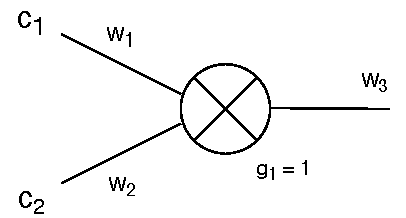
\includegraphics[width=\textwidth]{arith_circ/basic1.pdf} \caption{Basic
multiplication of two scalars} \label{fig:arith:basic} \end{subfigure}
\hspace{1cm}
	%
  \begin{subfigure}[b]{0.4\textwidth}
  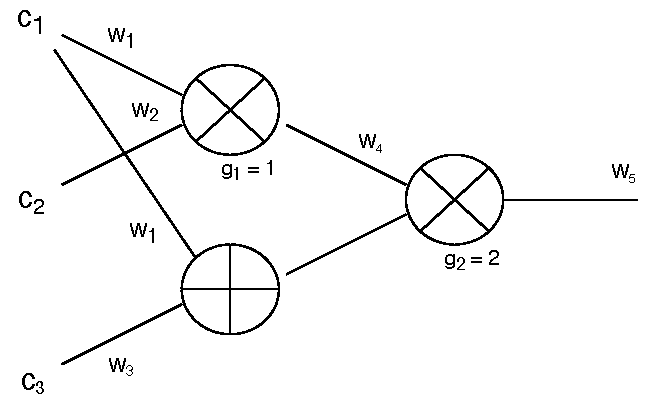
\includegraphics[width=\textwidth]{arith_circ/add_mult.pdf} \caption{Combined
addition and multiplication} \label{fig:arith:add_mult} \end{subfigure}
\caption{Arithmetic circuits} \end{center} \end{figure} 

In this circuit, we
identify one multiplication node (or gate) $g_1$, that has one left wire, $w_1$,
one right wire $w_2$ and one output wire $w_3$.\\ The $w_i$s are constants that
we will be trying to solve with the circuit. The first rule is that the wires
after incoming constants are assigned those constants, so in this case:
$$c_1\rightarrow w_1,\,\,c_2\rightarrow w_2,$$ Now we say that the circuit is
\emph{satisfied} of \emph{valid} or \emph{legal} if $w_3$ is assigned the
constant $c_3$, and we have $c_3=c_1\cdot c_2$. In general, for a circuit with
$W$ wires, an array of constants $$(c_1,\ldots,c_W)$$ is a valid assignment for
that circuit if every $c_i$ is assigned to $w_i$ in a way that for every output
wire, the assigned constant equals the result of the arithmetic operation on the
assigned constants of the incoming wires.\\ This may sound extremely trivial, to
the point that it feels like nothing is going on, which admittedly is almost the
case. But we will go on and make this a little bit more complicated.\\ \\ For
later purposes, we are going to label the wires of a general circuit in a
specific way, in a way that may sound random, but will make sense later when we
get closer to the polynomial business.\\ In our arithmetic circuit,
multiplicative gates are special: we only label multiplicative gates with $g_i$,
and only wires coming out of a multiplicative gate will be labeled, where we
think of the very incoming constants as being multiplication gates themselves
(the result of $c_i \cdot 1$). Next, we introduce the rule that, when from a
node\footnote{we use the name node and gate interchangeably} more than one wire
springs into another node, we will still think of this (bundle of) wire as one
wire with one label. Again, the very incoming variables of the circuit will for
this rule be thought of as nodes.

%------------------------------------------------------------------%
\subsection{Making Polynomials (Quadratic Arithmetic Program)}
%------------------------------------------------------------------%

With these rules in hand, we are ready to start cooking up the functions we
need. First, we introduce the \emph{target polynomial} $t(X)$ as follows:

\begin{defn}\label{def:arith_circ}
For an arithmetic circuit over $\mathbb{F}$ with $\mathcal{M}$ the set of multiplicative gates, $|\mathcal{M}|=M$, the \emph{target polynomial} $t(X)$ is defined as
\be
t(X)=\prod\limits_{i=1}^{M}\,(X-s_i),
\ee
for distinct $s_i\in\mathbb{F}$.
\end{defn}

That is with each multiplicative gate $g_i$ we associate a field element $s_i$
where all $s_i$'s are distinct. Note that for this definition to make sense we
need $M\leq |\,\mathbb{F}\,|$.\\ Next, we are going to cook up three more
polynomials: $\ell(X)$, $r(X)$ and $o(X)$, that will be associated to the left,
right and output wires of the circuit respectively.\\ First, recall that only
output wires of a multiplicative gate gets a label. When we identify all the
\emph{left} incoming wires of a gate $g_i$, we will however count all wires that
go into it either directly (coming directly from a multiplicative gate) or
\emph{indirectly} (passing first through one or several additive gates before
reaching $g_i$.) We will call the set of all these incoming left wires of gate
$g_i$: $\mathcal{I}_{i,L}$, and similarly the set of such wire for the right
incoming wires is written as $\mathcal{I}_{i,R}$.\\ Take for example the circuit
in figure \ref{fig:arith:add_mult}. There we have: $$\mathcal{I}_{2,L} = \{w_4
\},\,\, \mathcal{I}_{2,R} = \{w_1,w_3\}.$$ Finally, let $c_{i,L,k}$ denote the
fixed scalar that is multiplied with over a wire $w_k\in\mathcal{I}_{i,L}$, so
that for every output $w_g$ of a gate $g_i$ we can write

\be
w^{out}_i = \left(\sum\limits_{k\in \mathcal{I}_{i,L}} c_{i,L,k}\cdot w_k
\right)\cdot \left(\sum\limits_{k\in \mathcal{I}_{i,R}} c_{i,R,k}\cdot w_k
\right) 
\ee

Still in circuit \ref{fig:arith:add_mult}, this translates to
$$w_5 = \left(w_4 \right)\cdot \left(w_1+w_3\right)$$
For a gate $g_i$ we will now set the output polynomial $o_i(X)$ by demanding that

\be
o_i(s_j)=\delta_{ij}
\ee

that is: $o_i(s_j)=1$ iff $i=j$ and $o_i(s_j)=0$ otherwise. One
solution\footnote{This solution is by no means unique, but it is unique in this
degree $d=M-1$. Any positive power of $o_i(X)$ solves the condition also, or we
could multiply with any polynomial $f(X/s_i)$ that has no constant term.} is:

\be
o_i(X)=\prod\limits_{m\neq i}\frac{X-s_m}{s_i-s_m}.
\ee

Also, for all wires in $\cI_{g,L/R}$ we define polynomials by
demanding\footnote{Note that by abuse of notation, when we write $k\in
\cI_{j,L/R}$, we do not mean that $k$ is an actual wire $w_q$, but $k$ is the
index $q$ of that wire.}

\bea
\ell_i(s_j)=c_{j,L,i}\;\;\text{ for $k$ in } \cI_{j,L},\;\; 0 \text{ otherwise} 
\\
r_i(s_j)=c_{j,R,i}\;\;\text{ for $k$ in } \cI_{j,R},\;\; 0 \text{ otherwise} 
\eea

The solution to these is straightforward although slightly more involved. We
write down a solution for the case of $M=2$:

\bea
\ell_1(X)=&&\frac{c_{2,L,1}-c_{1,L,1}}{s_2-s_1}X+\frac{s_1c_{2,L,1}-s_2c_{1,L,1}}{s_1-s_2}\\
\ell_3(X)=&&c_{2,L,3}(X-s_1)
\eea

and similar for $r_i(X)$.\\
Now we define the following sums:

\bea
o(X)=&&\sum_{i=1}^W c^{out}_i o_i(X)\\
\ell(X)=&&\sum_{i=1}^{W} c_i\ell_i(X)\\
r(X)=&&\sum_{i=1}^{W} c_ir_i(X),
\eea

where $W$ is the number of wires in the circuit, $(c_1,\ldots,c_W)$ is an
assignment to the circuit, and $c_i^{out}$ is the assignment to the wire coming
out of gate $g_i$. Finally, we define

\be
p(X)=\ell(X)\cdot r(X)-o(X).
\ee

This polynomial $p(X)$ will play the central role in the protocol: it's the
function \bP will claim to know. This is due to the following observation: The
construction of $o(X)$, $\ell(X)$ and $r(X)$ is such that, when evaluated at any
of the $s_i$, we can readily check that, iff $(c_1,\ldots,c_W)$ is a valid
assignment, then:

\be
p(s_i)=\ell(s_i)\cdot r(s_i) - o(s_i) =0,
\ee

or in other words $p(X)$ has at least all the roots of the \emph{target
polynomial} $t(X)$, or: $t(X)$ \emph{divides} $p(X)$: To set up the protocol, we
need the following theorem

\begin{thm}
An assignment $(c_1,\ldots,c_W)$ to a circuit with $W$ wires is valid if and
only if its \emph{target polynomial} $t(X)$ divides $p(X)$:

\be
t(X)|\,p(X)
\ee

\end{thm}

Hence, it is enough for \bP to prove to \bV that it knows $p(X)$ such that
$t(X)|p(X)$.\\ We can think of the components $\ell_i(X)$ as spanning up a
vector $\vec{\ell}$ (as similar for $r_i(X)$ and $o_i(X)$). Then, for an
arithmetic circuit $C$, we sometimes refer to the collection 

\be
Q(C)=\left(\vec{\ell},\vec{r},\vec{o},t(X)\right)
\ee 

as the \emph{Quadratic Arithmetic Program} of the circuit $C$.

%------------------------------------------------------------------%
\subsection{Naive approach}\label{sec:circuits:protocol}
%------------------------------------------------------------------%

The task for \bP is now to convince \bV that it knows $p(X)$ s.t. $t(X)|p(X)$.
The input for the protocol will be an arithmetic circuit $C$. Before going
further with a proper zk-SNARK protocol, we will first introduce a naive
attempt, and see what's wrong with that.

The first thing that comes to mind when trying to come up with a
(zero-knowledge) proof of knowledge for \bP to convince \bV that is knows a
$p(X)$ s.t. $t(X)|p(X)$ for some given $t(X)$ is to just cook up a version of
the \hyperlink{box:schnorr}{Schnorr protocol}, but in a version that would allow
the secure communication of a polynomial. For an integer $n$, we know how to do
a secure transfer to a verifier of the wire: we take a finite cyclic group $G$
that is generated by $g$ and we send $y=g^n$ to \bV. The verifier can then
manipulate $y$ using homomorphicity and check it has certain properties, without
learning what $n$ is -- solving the discrete logarithm is in NP.\\

For a polynomial $p(X)$ we could do something very similar. Here's what the
equivalent of the Schnorr Sigma protocol for a proof the knowledge of a
polynomial $p(X)=\sum_{i=0}^{d}c_iX^i$ of degree $d$, with coefficients in
$\mathbb{F}$ and such that $t(X)|p(X)$, would look like.

\begin{enumerate}
	\item Set-up: \be bp = (p,G,g) \ee
	This is the agreed upon data that will be used throughout the protocol.
	\item \bV: takes $s\leftarrow\mathbb{F}$; sends to \bP: $\{g^{s^i}\}_{i=0}^{d}$
  \item \bP: computes $h(X)=\frac{p(X)}{t(X)}$; computes
    $g^{p(s)}=\prod\limits_{i=0}^d\left(g^{s^i}\right)^{c_i}$ and similarly
    computes $g^{h(s)}$; sends $(g^{p(s)},g^{h(s)})$ to \bV
	\item \bV: checks that $g^{p(s)}=\left(g^{h(s)}\right)^{t(s)}$. If true, it accepts the claim; if false rejects.
\end{enumerate}

There are multiple ways in which this protocol is not satisfactory.\\ 

First, the prover's claim isn't very impressive. To know a degree $d$ polynomial
such that a given $t(X)$ of degree $d'<d$ divides it, isn't hard. We can just
take $t(X)$ and multiply by any degree $d-d'$ polynomial, so we need more
properties on $p(X)$ to make this hard, as we will later -- or already have in
the previous section. Still, this example is instructive, as it does contain the
gist of the eventual protocols.\\ 

Second, although this protocol is \emph{complete}, it is not \emph{sound}, that
is: there are ways for a malicious \bP to convince \bV of a false proof. For
example, without knowing any polynomial at all, \bP could just take a random
$r\leftarrow \mathbb{F}$ and send the pair $(g^{t(s)\cdot r},g^r)$ to \bV. This
would be accepted. We need to cook up a way to force \bP into correctly
following the protocol, or at least having a check to find out if it has.\\

Thirdly, the protocol is not zero-knowledge, and there are ways for \bV to
extract information about $p(X)$: given $g^{p(s)}$, it can brute-force try
$c_i$'s to land at that result, with $g^{\sum_{i}c_is^i}$.\\ The first problem
is in a way addressed in the previous section, as we will eventually not be
interested in just the naked polynomial $p(X)$ but in it's composition in terms
of $\ell(X)$, $r(X)$ and $o(X)$, in a way that its properties will be hard
enough be be non-trivial for the prover.\\ The second and third problem need a
bit more attention. We'll introduce techniques to address these two issues right
away.
\newline

%------------------------------------------------------------------%
\hypertarget{box:np}{\hspace{-0.5cm}}\setlength{\fboxsep}{15pt}\hypertarget{box:schnorr}\shadowbox{\parbox{13.3cm}{\centerline{\textbf{Schnorr
    Protocol and the Fiat-Shamir Heuristic}}\vspace{5pt} The Schnorr protocol is
    probably the simplest and most instructive example of a \emph{proof of
    knowledge}. The set-up is: given a finite cyclic group $G$ of order $p$,
    generated by $g$, a prover \bP wants to prove to \bV that, given $y\in G$,
    it knows $x$ such that $y=g^x$. The proof goes in three steps:
\begin{enumerate}
	\item \bP takes a random $r\leftarrow G$ and sends $t=g^r$ to \bV
	\item \bV takes a random $c\leftarrow G$ and sends it to \bP
	\item \bP computes $s=r+cx$ and sends $s$ to \bV
\end{enumerate}
After this communication, \bV accepts \bP\!\!'s statement if $g^s=t\cdot y^c$. 
Such protocols are sometimes called Sigma protocols (drawing the 3-steps, it
resembles the Greek capital Sigma). Note, however, that \bP can also just take a
random $x'$ that does not in fact solve the discrete log problem at hand, and it
still has some chance of being accepted by \bV. This probability is one over the
size of the challenge space where $c$ is taken from. \\We'll just state here
that this protocol only zero-knowledge when the verifier's challenge space
(where $c$ is taken from) is small, e.g. when $c\in\{0,1\}$. In this scenario,
however, for the verifier to be properly convinced of \bP\!\!'s statement (it is
zero-knowledge, but not ``sound''), and the protocol needs to be run many times
to satisfy the soundness requirement -- not a practical situation.\\
This protocol has another disadvantage: it is ``interactive'' -- both \bP and
\bV need to be on-line and need to exchange data. We can render this protocol
non-interactive as follows: we replace step 2. by:
\begin{enumerate}
	\setcounter{enumi}{1}
  \item \bP computes $c=H(g,y,t)$ and sends it to \bV, where $H$ is a random
    oracle, or cryptographic hash function, e.g. $H=\text{sha256}$ as of
    writing.
\end{enumerate} 
Now the Sigma protocol is turned into a non-interactive proof of knowledge. This
is a very common procedure, and is sometimes called the Fiat-Shamir Heuristic.
  } }
%------------------------------------------------------------------%


%------------------------------------------------------------------%
\subsubsection{Soundness by shifting}
%------------------------------------------------------------------%

The gist of the soundness problem of our naive protocol is this (where we use a
number case first and discuss polynomials later):\\ \indent \bV wants to pick a
$g$, and then have \bP take a value $c$ -- that's only known to \bP --, encrypt
it with $g$ (i.e. compute $g^c$), and send $g^c$ back to \bV\!\!. In the
process, \bP wants to keep $c$ hidden from \bV\!\!.\\ Now, how does \bV check
that indeed \bP followed the instructions, and not just sent some bogus value?
The simplest way would of course be for \bP to just supply $c$ itself, but \bP
will not agree on this as it is trying to achieve zero-knowledge. A better
solution is this little protocol:\\ First, \bV takes a random $\alpha$, and
sends $(g,g^\alpha)$ to \bP. Then, it asks \bP to encrypt its secret $c$ using
both $g$ and $g^\alpha$, and send both encryptions
$(z,z')=(g^c,\left(g^{\alpha}\right)^c)$ back. Now, \bV can check if indeed
$z^\alpha=z'$. If that is the case, \bV can conclude that indeed \bP followed
the instructions.\\ That \bV may conclude so is based on the ``Knowledge of
Coefficient Assumption'' (KCA). This assumption basically states that there is
no efficient way for a prover \bP to, given a pair $(x,x^\alpha)$, send back a
pair $(z,z')$ that also obeys $z^\alpha=z'$, except from -- rather trivially --
returning $(x^c,\left(x^\alpha\right)^c)$ for some choice of $c$. That is: when
\bP gives back that pair it \emph{knows} the coefficient $c$.\\ \newline In
making the zk-SNARK, we're not exchanging numbers but rather polynomials, so we
need to generalize this protocol to allow for this case also. This is
straightforward, and we give here the updated protocol that includes the shift:
\begin{enumerate}
  \item \bV: takes an $s\leftarrow\mathbb{F}$ and an
    $\alpha\leftarrow\mathbb{F}$; sends to \bP: $\{(g^{s^i}\!,\, g^{\alpha
    s^i})\}_{i=0}^{d}$
  \item  \bP: computes $h(X)=\frac{p(X)}{t(X)}$; computes
    $g^{p(s)}=\prod\limits_{i=0}^d\left(g^{s^i}\right)^{c_i}$ and similarly
    computes $g^{h(s)}$; it also computes $g^{\alpha
    p(s)}=\prod\limits_{i=0}^d\left(g^{\alpha s^i}\right)^{c_i}$; sends
    $(z_p,z_{\alpha p},z_h)=(g^{p(s)},g^{\alpha p(s)},g^{h(s)})$ to \bV
  \item \bV: checks that $z_p=z_h^{\,t(s)}$ and that also
    $z_p^{\,\alpha}=z_{\alpha p}$. If true, it accepts; if false rejects.
\end{enumerate}

%------------------------------------------------------------------%
\subsubsection{Zero-knowledge by shifting}
%------------------------------------------------------------------%

The protocol is not yet zero-knowledge: the verifier receives $g^{p(X)}$ and
although it is hard to obtain $p(X)$, it is possible, given enough computation
time and strength.\\ With the previous section in mind, this problem is actually
pretty easy to address. In that protocol, instead of sending $(z_p,z_{\alpha
p},z_h)$, \bP could just first sample a random $\delta\leftarrow\mathbb{F}$, and
send to \bV the triplet $(z_p^\delta,z_{\alpha p}^\delta,z_h^\delta)$. That way,
the protocol is still sound and complete, but now it's also zero-knowledge. 

\subsubsection{Non-interactive by pairing}

That our protocol is interactive is still problematic, and there is not yet a
straightforward application of the \hyperlink{box:schnorr}{Fiat-Shamir
heuristic}. A first attempt is to introduce a third, central party that
everybody -- both \bV and \bP -- trust. From a cryptocurrency point of view this
is of course not an interesting definitive solution, but we'll touch upon it
here as it is an instructive example to build on, and also immediately
introducing the trusted set-up with a ``nearly-trustless'' set-up.\\ First, lets
call the trusted party \bT. This is what the first part of our non-interactive
protocol with trusted set-up, for proving \bP knows a degree-$d$ polynomial
$g(X)$ with $t(X)|g(X)$ for public $t(X)$, looks like:

\begin{enumerate}
\item Set-up: $bp=(p,G,g)$
\item \bT takes $s,\alpha\leftarrow\mathbb{F}$; computes
  $(g^\alpha,g^{s^i},g^{\alpha s^i},g^{t(X)})$; makes this public as follows:
\bea \text{pk} =(g^{s^i},g^{\alpha s^i}) \\
 \text{vk} = (g^{t(s)},g^{\alpha})
 \eea
 where we call pk and vk the proving key and verification key respectively
 \item \bT deletes $(s,\alpha)$
\end{enumerate}
With this set-up, we aim at a scenario where \bV needs to do nothing but check
something, and needs no communication with \bP. The idea is that, with the help
of \bT\!'s proving key, \bP computes $g^{p(s)}$, $g^{\alpha p(s)}$, $g^{h(s)}$,
and then \bV gets to verify just like before, now using the verification key.
\bV needs one more instrument to facilitate this verification: a bilinear
pairing.\\

\begin{defn}\label{def:pairing}
A map $e:G_1,G_2\rightarrow H$, with $G_1,G_2,H$ finite groups, is called bilinear if 
$$e(g_1^n,g_2^m)=e(g_1,g_2)^{mn}.$$
We call $e$ a \emph{pairing} if it is non-degenerate (there's no $g\in G_1$ such that $e(g,g')=1$ for all $g'\in G_2$) and if it furthermore can be efficiently computed.
\end{defn}

It is first of all not obvious such a pairing should exist for every triplet of
groups $(G_1,G_2,H)$. We will however, in cryptography, be interested in the
scenario where we have explicit construction of such a pairing in hand. This is
the case when we restrict the groups to descend from certain elliptic curves,
where there is such a construction called the Tate pairing. It is beyond the
scope of this text to delve deeper into elliptic curves and their pairings, also
because there are great texts out there, so throughout we will think of the
groups and the pairings as given.\\ With this pairing, that will be a given, we
are ready to complete the verification step of our zk-snark:
\begin{enumerate}
	\item Set-up: $ bp=(p,G,g,e)$ with $e:G\times G\rightarrow G$
	\item After the \bT has generated the proving key and verification key as above, and \bP used pk to compute $\pi=(g^{\delta p(s)},g^{\delta\alpha p(s)},g^{\delta h(s) })$, a triplet that \bV will parse as $\pi=(g^p,g^{\alpha p},g^h)$.
	\item \bV checks that $e(g^p,1)=e(g^t,g^h)$ and $e(g^{p'},1)=e(g^p,g^\alpha)$
\end{enumerate}

With this last step, we solved a lot of our problems. There are two more
problem. First, is the trusted set-up. From a crypto coin point of view, this is
serious and one might say we have in the process threw out the baby with the
bathwater. One way to solve this is to not introduce on trusted party, but
introduce a lot of them, and start the protocol with a ceremony, where all
trusted party members participate in generating the proving key and verification
key. There is a neat way that makes sure the keys will be corrupt only is
\emph{all} participants of the ceremony all malevolent, that is trusting one out
of the entire community would be enough (REF HERE). Although this is definitely
an improved scenario, it still is not ideal. This process can be lengthy or
messy, and it makes it hard to refresh the keys if needed, so we will look for
another approach.  Secondly, we still have the problem of triviality: the prover
is still not proving anything fascinating.
We will address this issue now, introducing the Pinocchio protocol.
% (REFERENCE https://www.math.uwaterloo.ca/~ajmeneze/publications/pairings.pdf).



%------------------------------------------------------------------%
\subsection{Pinocchio Protocol}
%------------------------------------------------------------------%

We now have everything in place to start introducing some actual useful
protocols, starting with the Pinocchio
protocol\cite{parno2016pinocchio}. The Pinocchio protocol is the first
practical zk-Snark protocol that was published. It contains the
ingredients that we introduced in the previous sections, but also
address the last standing open challenge. Whereas in the previous
section, the prover was not very impressive in its claim; the Pinocchio
protocol upgrades that scenario, really making the protocol about the original
problem: proving knowledge of some constants in a relation. This protocol will
be interactive and can be made non-interactive by the trusted party method as
described in the previous section. We will follow the notation of
\cite{parno2016pinocchio} quite closely, so that the reader can easily switch to
that reference. Like any public verifiable computation scheme, the protocol will
have three steps: Key generation ($(pk;vk)\leftarrow KeyGen(F)$), Compute
($(y;\pi_y)\leftarrow Compute(pk,u)$) and Verify $((0;1)\leftarrow
Verify(vk,u,y,\pi_y))$.\\
The set-up will be that we have some elementary relation $F$ with a total of $N$
input/output variables in the field $\mathbb{F}$.

\setlength{\fboxsep}{10pt}\fbox{\parbox{11cm}{\centerline{\textsc{Pinocchio
    protocol}}\vspace{-2pt}

    {\tiny

        \centerline{\rule{11cm}{1pt}} \vspace{-2pt} Input: Relation $F$ with $N$
        input/output variables $c_i$. \vspace{-7pt}\\ \centerline{\rule{11cm}{0.2pt}} 
\begin{enumerate} 
  \item Set $bp = \left(p,G,G_T,g,e\right)$, where $p$ is a prime number,
    $G,G_T$ are finite groups, $|G|=p$ and $g$ generates $G$: $\langle g
    \rangle=G$, and $e$ a non-trivial bilinear map $e:G\times G\rightarrow
    G_T$.  
  \item Convert $F$ into an arithmetic circuit $C$ and construct the
        corresponding degree-$d$, size-$m$\footnote{recall that with
        \emph{degree} we mean the number of multiplicative gates and hence
        degree of $t(X)$ and the
    \emph{size} $m$ equals the number of wires in the circuit} QAP
    $Q(C)=\left(t(X),\vec{\ell},\vec{r},\vec{o}\right)$. Set $I_{mid} =
    \{N+1,\ldots,m \}$ 
  \item \textbf{Key Generation} $SRS=(pk,vk)\leftarrow \text{KeyGen}(F)$\\ Sample
  $s,r_\ell,r_o,\beta,\alpha_\ell,\alpha_r,\alpha_o,\gamma\leftarrow\mathbb{F}$.
  Set $r_o=r_\ell\,r_r$ and define $g_\ell=g^{r_\ell}, g_r=g^{r_r}, g_o=g^{r_o}$.
  Now define the proving key $pk$ as:
  \begin{align}\nonumber
  pk=\big(\{g_\ell^{\ell_k(s)}\}, \{g_r^{r_k(s)}\}, \{g_o^{o_k(s)}\},
    \{g_\ell^{\alpha_{\ell} \ell_k(s)}\}, \{g_r^{\alpha_r r_k(s)}\}, \\\nonumber 
    \{g_o^{\alpha_o o_k(s)}\}, \{g^{s^i}\}, \{ g_\ell^{\beta\ell_k(s)}g_r^{\beta
  r_k(s)}g_o^{\beta o_k(s)}  \}\big)_{k\in I_{mid},\, i\in [0,\ldots, d]}
  \end{align}
  and the verification key $vk$ as:
\begin{align}\nonumber
  vk = \left(
    g,g^{\alpha_{\ell}},g^{\alpha_r},g^{\alpha_o},g^\gamma,g^{\beta\gamma},g_o^{t(s)},\{
    g_\ell^{\ell_k(s)}g_r^{r_k(s)}g_o^{o_k(s)}
  \}_{k\in[0,\ldots,N]}
\right)
\end{align}
\item \textbf{Compute} $(y,\pi_y)\leftarrow \text{Compute}(pk,u)$
  Given some input $u$ for the relation $F$, the prover evaluates the arithmetic
  circuit to obtain $y\leftarrow F(u)$ and thus learns the values
  $\{c_i\}_{i\in[0,\ldots,m]}$ that are assigned to the wires.\\
  Prover computes $h(X)$ such that $p(X)=h(X)t(X)$ and cooks up the proof
  $\pi_y$:
  \begin{align}\nonumber
   \pi_y = \big(
     g_\ell^{\ell_{mid}(s)}, g_r^{r_{mid}(s)}, g_o^{o_{mid}(s)},
     h^{h(s)}, g_\ell^{\alpha_\ell \ell_{mid}}, g_r^{\alpha_r r_{mid}(s)}, \\\nonumber
g_o^{\alpha_o
     o_{mid}(s)}, g_\ell^{\beta \ell_{mid}(s)}g_r^{\beta r_{mid}(s)}g_o^{\beta o_{mid}(s)}
    \big) 
  \end{align}
  where $\xi_{mid}(x)=\sum\limits_{k\in I_{mid}} c_k\, \xi_k(x)$ for
  $\xi\in\{\ell,r,o\}$

\item
  \textbf{Verify} $\{0,1\}\leftarrow \text{Verify}(vk,u,y,\pi_y)$\\
The verifier parses the proof $\pi_y$ as
\[\pi=(g^L,g^R,g^O,g^H,g^{L'},g^{R'},g^{O'},g^Z).\] Computes:
$g_\ell^{\ell_{I/O}(s)}=\prod\limits_{k=0}^N\left(g_\ell^{\ell_k(s)}\right)^{c_k}i,
c_0=1$
(and similar for $r,o$). Now checks:
\begin{itemize}
  \item[--] Divisibility: \[ e(g_\ell^{\ell_{I/O}(s)}g^L, g_r^{r_{I/O}(s)}g^R) =
e(g_o^{t(s)},g^H)e(g_o^{o_{I/O}(s)}g^O,g)  \]
\item[--] Shifting: \[ e(g^{L'},g) = e(g^L,g^{\alpha_\ell})\; \text{ (and same for R
  and O)} \]
\item[--] Coefficients: \[ e(g^Z,e^\gamma) = e(g^Lg^Rg^O,g^{\beta\gamma}) \]
\end{itemize}
\end{enumerate}  }  } }
\newline
\newpage
This is the Pinocchio protocol. It is the first bona-fide zk-SNARK. It does now
prove something NP-hard, but it still has some problems.\\ The set-up is still
trusted. Now, we can still upgrade this trusted set-up to one where we
distribute the trust over some network of clients, up to the point where we only
need to trust one out of many to trust the entire set-up. One thing we would
however like to introduce is some manner of being able to update the trusted
set-up. Currently, we first have to start some ceremony, where one group of
clients first has to generate the set of keys \[SRS=(pk,vk).\footnote{This set
is commonly referred to as the SRS: the structured reference string}\] Once this
SRS is constructed, however, later in the process it cannot be altered. This is,
from a security/crytpo point of view somewhat counter-intuitive and we would
like a scenario where this SRS can be updated at any time without hassle. Sonic
will do this, based on the ideas of Groth et all [REF]. We will now introduce
Sonic.

%--------------------------------------- ---------------------------%
\section{Sonic }\label{sec:sonic}
%------------------------------------------------------------------%

Sonic is an improvement of the Pinocchio protocol. Its methods aren't radically
different but there are some new ingredients that we will list. We will not go
into detail about this, but the protocol we will introduce here has one
shortcoming that will be fixed in the next section. This has to do with
computation times. We did not talk about this too much, but for zk-SNARKs to be
practical they need to be fast. SuperSonic will basically be a speed-improved
version of Sonic.\\ The new ingredients, that are referred to as Building Blocks
in [REF], are:
\begin{itemize}
  \item \textbf{Bilinear Groups} The form of $bp$ is:
    $bp=\left(p,G_1,G_2,G_T,e,g,h \right)$, where $G_1=\langle g \rangle$,
    $G_2=\langle h \rangle$, $G_T=\langle e(g,h)\rangle$, and $G_1$ and $G_2$
    are such that there is no
  \item \textbf{SRS} The general form of the SRS is \[SRS=\left\{
    \{g^{x^i}\}_{i=-d}^{d},\,\{g^{\alpha x^i}\}_{i=-d,i\neq
0}^{d},\,\{h^{x^i},h^{\alpha x^i}\}_{i=-d}^{d},\, e(g,h^\alpha) \right\}\]
	Note the negative powers, and also that $g^\alpha$ is not part of the SRS.
  \item \textbf{Polynomial Commitment Scheme} It uses a \emph{polynomial
    \hyperlink{np:box}{commitment scheme}}. We explain this scheme in subsection
    (\ref{subsec:poly}).
\end{itemize}
The way the constraints are mapped to a polynomial is also different in Sonic.
We will now discuss these new ingredients in some more detail. 

\subsection{System of Constraints}
The way that the constraint relation $F$ is packed, is a little different in
Sonic. \\ \newline We start with three vectors,
$\mathbf{a},\mathbf{b},\mathbf{c}\in\mathbb{F}^n$, such that

\be\label{eq:mult}
\mathbf{a}\circ\mathbf{b}=\mathbf{c},
\ee

where $\circ$ means component-wise multiplication. To accommodate the linear
constraints, we further introduce $Q$ linear constraints

\be\label{eq:constraint}
\mathbf{a}\cdot \mathbf{u}_q+\mathbf{b}\cdot
\mathbf{v}_q+\mathbf{c}\cdot\mathbf{w}_q=k_q
\ee

where $q=1,\ldots,Q$ and
$\mathbf{u}_q,\mathbf{v}_q,\mathbf{w}_q\in\mathbb{F}^n$, $k_q\in \mathbb{F}_p$.
We will quickly discuss a couple of examples to illustrate how this works.

\begin{itemize}
  \item Even though it looks slightly patronizing, let's start with the very,
    very most simple relation. A linear relation in one variable $x_1$ that is
    known to the prover: \[x_1=r\] for some $r\in \mathbb{F}_p$. Now of course,
    this example is trivial, as the solution is equal to the relation itself! It
    is however instructive to translate this to the language of Sonic's system
    of constraints. We should think of this as already having one
    ``multiplicative gate", and $n=1$. The multiplicative relation is $a_1\cdot
    b_1=c_1$, so our relation should really be seen as $1\cdot b_1=r$. So
    there's a left input variable $a_1$ that's constrained to $a_1=1$, there's a
    right input $b_1$ (that we labeled $x_1$ in our formulation) that has no
    constraint, and finally there's an output $c_1$ constrained to $c_1=r$. So,
    $Q=2$, and $(u_1,v_1,w_1;k_1)=(1,0,0;1)$ and $(u_2,v_2,w_2;k_2)=(0,0,1;r)$.
    Note that the system is not unique. A system that describes the same
    relation is $(u'_1,v'_1,w'_1;k'_1)=(1,0,0;1)$,
    $(u'_2,v'_2,w'_2;k'_2)=(0,1,0;r)$ and $(u'_3,v'_3,w'_3;k'_3)=(0,0,1;0)$.
    Also, we have the freedom of picking what we call left and right inputs. We
    will call all such systems that describe the same relation equivalent.
  \item The next simplest case is arguably that of a system of two variables
    $x_1,x_2$ that obey a linear constraint $x_1+x_2=r$. In this new system, we
    can identify the vectors as
\[ \mathbf{a}=\bem a_1 \\ a_2 \eem\!,\, \mathbf{b}=\bem b_1 \\ b_2 \eem\!,\,
\mathbf{c}=\bem c_1 \\ c_2 \eem  \]
Without loss of generality, we will identify our variables $x_{1,2}$ with
$b_{1,2}$ respectively. Will will then consider out system consisting of having
two multiplicative gates that our not connected, with some additional
constraints on top.\\
The first constraint is $a_1=1$. So: $\mathbf{u}_1=\begin{psmallmatrix} 1\\0
\end{psmallmatrix} $ and $\mathbf{v}_1=\mathbf{w}_1=0$, $k_1=1$. The second is $a_2=1$:
$\mathbf{u}_2=\begin{psmallmatrix} 0\\1
\end{psmallmatrix} $ and $\mathbf{v}_2=\mathbf{w}_2=0$, $k_2=1$. Then we have
$b_1-c_1=0$ and $b_2-c_2=0$: $u_3=0$ and $\mathbf{v}_3=\begin{psmallmatrix} 1\\0
\end{psmallmatrix} $, $\mathbf{w}_3=\begin{psmallmatrix} -1\\0
\end{psmallmatrix} $, $k_3=0$ and similar for $q=4$. Then finally we have the
actual additive constraint: $b_1+b_2-r=0$: $u_5=0$,
$\mathbf{v}_5=\begin{psmallmatrix} 1\\1
\end{psmallmatrix} $, $w_5=0$ and $k_5=r$.     
\end{itemize}
\newpage
These examples, that touch upon just the most trivial of cases, show that these
arithmetic circuits really pull apart their elementary relations to their most
primitive roots, and in the process make them look quite intricate cumbersome.\\
We will now move on tho show how this, in Sonic, is translated into polynomials.

\subsection{Multivariate Polynomials}

From the relations (\ref{eq:mult}) and (\ref{eq:constraint}) we will now proceed
to construct polynomials that will actually be used in the zero knowledge
protocol. 

\subsection{Polynomial Commitment Scheme}\label{subsec:poly}
	
\hypertarget{box:np}{\hspace{-0.5cm}}\setlength{\fboxsep}{15pt}\hypertarget{box:np}\shadowbox{\parbox{13.3cm}{\centerline{\textbf{Commitment}}\vspace{5pt}
    A commitment $\text{Com}(m)$ is a way for an actor \bP to take a secret
    message $m$, and seal it in a little protocol in a way that \bP is committed
    to $m$ until the end of the protocol. It is the digital equivalent of
    putting your message in a sealed envelope, such that before the end of the
    ceremony, $m$ stays hidden but can not be altered by \bP, as in the final
    step, the envelope will be opened to check if indeed \bP stayed committed to
    $m$. It should work such that, once \bP has filed the commitment, it can not
    change $m$ without someone noticing, while at the same time it should
    perfectly hide $m$ for anyone else involved.\\ The first thing you might
    think of is: use a random oracle/hash function. Indeed, this checks to
    stated requirements. It has the problem however of being one-time useful
    only. Suppose a ceremony includes \bP making a commitment to some small
    integer $n$, committed to with $\text{Com}(n)=\text{sha}(n)$. At the end,
    \bP reveals $n$ and anyone can check that indeed the hash function checks
    out. However, any time in future this same integer pops up, anyone will
    recognize the hash function, and the commitment is not hiding the message
    any more.\\ We can solve this by first raking a random string $r$,
    joining/concatenating it with $m$ as $r||m$; applying the hash,
    $\text{Com}(m)=\text{sha}(r||m)$, and at the end releasing both $r$ and $m$.
    If $r$'s sampling space is large enough this will do. The practical problem
    is that this scheme is not \emph{homomorpihc}: it doesn't obey
    $\text{Com}(m_1\cdot m_2)=\text{Com}(m_1)\cdot \text{Com}(m_2)$. This is needed
    if we want to be able to update out commitment.
    A homomorphic, hiding commitment scheme is given by \emph{Pedersen's
    commitment scheme}:
\begin{enumerate}
  \item Set-up: A large prime $p$, and a $q|p-1$ are generated, as well as
    the group $\mathbb{Z}_{q}$ generated by $g$, with
    $\mathbb{Z}_q\subset\mathbb{Z}_p^*$. A second generator $h$ is chosen, and
    \bP can not know $a$ such that $g^a = h$.
    $(p,q,\mathbb{Z}_q,g,h)$ are all public: only $a$ is secret.
  \item Commit: \bP now \emph{commits} to an $m\in\mathbb{Z}_q$ by taking
    $r\leftarrow\mathbb{Z}_q$ and making public: \be c=g^mh^r \text{ mod }  p\ee
  \item Open: To, at the end of a ceremony, \emph{open} of \emph{reveal} the
    commitment, \bP publishes $(m,r)$.
\end{enumerate}
 } }


%------------------------------------------------------------------%
\section{Beyond Sonic}\label{sec:improv}
%------------------------------------------------------------------%


%------------------------------------------------------------------%
\addcontentsline{toc}{section}{References}
\bibliographystyle{alpha}
\bibliography{zk}

%------------------------------------------------------------------%
\end{document}
